\chapter{Diseño\label{sec:disenho}}

\section{Introducción}
Tras el análisis del panorama y las tecnologías \textit{big data} y, en especial, de las que van a ser utilizadas en este proyecto, en este apartado, se procederá con la explicación del diseño de la arquitectura \textit{big data} que, posteriormente, se implementará en un clúster doméstico.

En cuanto a la estructura de este apartado, en primer lugar procederemos a presentar la arquitectura del clúster, posteriormente se analizaran los \textit{insights} del proyecto y las fuentes que se utilizarán.

\section{Arquitectura del sistema}
\subsection{Modo distribuido o multinodo \label{disMultinodo}}
En este modo de ejecución se cuenta con más de una máquina para ser utilizada por el sistema, siendo la configuración utilizada en la gran mayoría arquitecturas \textit{big data} que se utilizan. 

En este tipo de ejecución se cuenta con una máquina que hará de maestro y distribuirá las tareas sobre el resto de nodos, los esclavos, y ella misma, para lograr la máxima eficacia de procesamiento. Es decir, el maestro creará un objeto \textit{SparkContext} que será el que distribuya los trabajos entre los nodos conectados y recogerá los resultados, como se muestra en la figura \ref{fig:clusterSpark} \cite{clusterfoto}.

\begin{figure}[htp!]
	\centering
	\caption{Modo distribuido o multinodo de \textit{Spark} \cite{clusterfoto}}
	\label{fig:clusterSpark}
	\includegraphics[scale=0.6]{graphics/sparkCluster}
\end{figure}

En este caso, la ventaja de esta configuración es la gran capacidad de procesamiento que se puede obtener, especialmente si las tareas ha realizar requieren gran cantidad de potencia de procesamiento, al disponer de la suma de los procesadores y de la memoria \gls{RAM} de los nodos del sistema.

La principal desventaja de este, que es su principal punto débil, se encuentra en la conexión entre los nodos, cuya calidad y velocidad afectará al rendimiento del sistema de forma muy importante. Es decir, el problema en los sistemas distribuidos proviene de la conexión de red entre los equipos, donde se pueden producir cuellos de botella en el envío de datos entre ellos. Estos pueden hacer que aunque la potencia teórica del sistema sea muy alta se obtengan malos rendimientos de procesamiento que hagan que el sistema no resulte rentable.

Otro de las desventajas de esta configuración es el coste de mantenimiento del conjunto de las máquinas y los dispositivos necesarios para mantener el clúster en funcionamiento.

\subsubsection{Clúster  \label{disDomestico}}
El número de máquinas que formarán este clúster serán dos, una de sobremesa que hará de maestro y esclavo y un portátil que hará de esclavo, un portátil y un sobremesa, como se puede observar en la figura \ref{fig:clusterDomestico}. Todos estos nodos estarán conectados a la red mediante cables Ethernet RJ45 Cat.5e UTP y un switch (TP-LINK TL-SG108) y contarán con Ubuntu 16.10 \cite{ubuntu} como versión del sistema operativo.

\begin{figure}[htp!]
	\centering
	\caption{Arquitectura del clúster doméstico}
	\label{fig:clusterDomestico}
	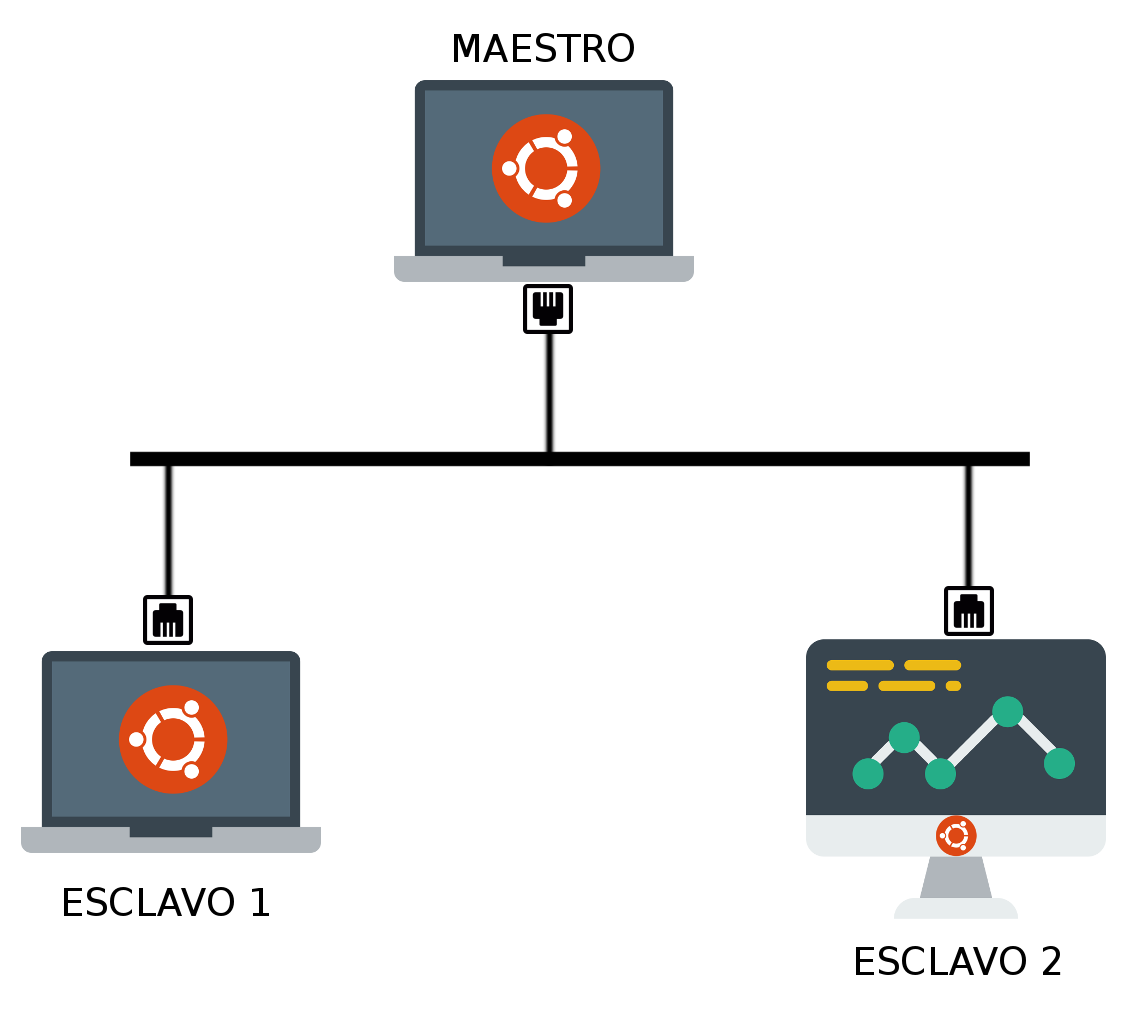
\includegraphics[scale=0.3]{graphics/clusterDomestico}
\end{figure}

\textit{Apache Hadoop} es la tecnología utilizada para montar este mecanismo de replicación mediante el uso de su sistema distribuido de ficheros (\gls{HDFS}) que resulta óptimo para esta configuración. Este mecanismo nos permitirá tener los datos en cada nodo del clúster y, así, lo único que circulará por la red serán las tareas que el maestro asigne a los esclavos y los resultados que estos obtengan tras su procesamiento. 

Esto evitará el tráfico que generaría transmitir los datos a procesar con la tarea asignada a los nodos esclavos, mejorando el rendimiento de la arquitectura.

\begin{figure}[htp!]
	\centering
	\caption{Esquema del sistema de replicación \gls{HDFS}}
	\label{fig:hdfs}
	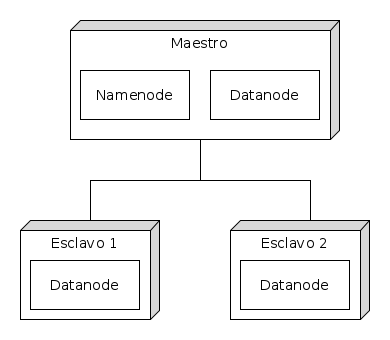
\includegraphics[scale=0.6]{graphics/hadoop}
\end{figure}

Como se aprecia en la figura \ref{fig:hdfs} que muestra el esquema del sistema de replicación, para su funcionamiento, en cada nodo se necesita un proceso \textit{datanode} ejecutándose, que será el que se encargue de el almacenamiento de los datos en la máquina. Además, para controlar el estado de los \textit{datanodes} se necesita un proceso \textit{namenode}, que se ejecutará en el nodo maestro.

\clearpage
\section{Insights del proyecto \label{insights}}
En este trabajo debido a que se realiza un proyecto real de análisis para una supuesta empresa de impartición de cursos, hay ciertas preguntas que se desean resolver a lo largo del proyecto, estás ``preguntas'' en ámbito de \textit{big data} se denominan \textit{insights} que iremos resolviendo hasta llegar al informe final.

\begin{itemize}
	\item ¿Cuáles son los lenguajes de programación más populares?
	\item En caso de regionalización ¿Qué países enfocar?
	\item ¿Qué idioma utilizan los programadores?
\end{itemize}

El primer paso para enfrentarnos a estos \textit{insights} será definir el termino ``popularidad'', para luego proceder a la resolución de estas cuestiones.


\subsection{Plan de proyecto}
El proyecto constará de diferentes fases donde primero implementaremos el clúster anteriormente mencionado.
Realizando un pequeño estudio preliminar encontramos que los programadores utilizan tres plataformas de forma predominante.
\begin{itemize}
 	\item \textbf{Stackoverflow \cite{stackoverflow}}. Esta plataforma está dedicada a que los programadores planteen dudas, que son resueltas por otro profesionales. Cada \textit{post} esta etiquetado con el lenguaje o tecnología sobre la que se realiza la cuestión.
 	
 	\item \textbf{GitHub \cite{github}}. Es un repositorio de versiones basado en \textit{Git} \cite{git}, el cual siguiendo la filosofía de \textit{open data} \cite{opendata} proporciona una \gls{API} desde la que se pueden descargar los eventos almacenados desde 2015 a través de \textit{GitHub Archive} \cite{githubArchive}.
 	
 	\item \textbf{Twitter \cite{twitter}}. Es una plataforma de comunicación bidireccional con naturaleza de red social (porque permite elegir con quien te relacionas). Cuyos mensajes están limitados a 280 caracteres. Aquí los usuarios publican sus opiniones personales o anuncios que consideran importantes. Proporciona una \gls{API} que permite obtener estos mensajes (\textit{tweets}) en tiempo real.
\end{itemize}

